\documentclass[tikz,border=6pt]{standalone}
\usepackage{amsmath,amssymb,mathtools,physics,bm,nicefrac,wasysym}
\usepackage{xcolor}

\definecolor{colone}{RGB}{180,60,60}
\definecolor{coltwo}{RGB}{60,110,180}
\definecolor{colthree}{RGB}{60,140,80}

\definecolor{accent}{HTML}{A13D2C}
\definecolor{accent2}{HTML}{2B5F6B}
\definecolor{muted}{HTML}{5A564F}
\definecolor{panel}{HTML}{F8F6F0}
\definecolor{linecol}{HTML}{D8D2C4}
\definecolor{ink}{HTML}{1E1C1A}
\definecolor{astroblue}{HTML}{1B4F72}
\definecolor{astrodark}{HTML}{17202A}
\definecolor{sunyellow}{HTML}{E8A33D}

\usetikzlibrary{calc,arrows.meta,positioning,decorations.pathreplacing,decorations.markings,angles,quotes,shapes.geometric}
\usepackage{tikz-3dplot}

\newcommand{\vecr}{\vec r}
\newcommand{\vecL}{\vec L}
\newcommand{\vecA}{\vec A}
\newcommand{\vecf}{\vec f}
\newcommand{\vecF}{\vec F}
\newcommand{\vecp}{\vec p}
\newcommand{\avg}[1]{\left\langle #1\right\rangle}
\newcommand{\vecx}{\vec x}
\newcommand{\hatn}{\hat n}
\newcommand{\rhat}{\hat r}
\newcommand{\phihat}{\hat\phi}
\newcommand{\thetahat}{\hat\theta}
\newcommand{\note}[1]{\textcolor{blue!60!black}{\textit{[#1]}}}

% Astronomical acronyms
\newcommand{\LST}{\mathrm{LST}}
\newcommand{\GST}{\mathrm{GST}}
\newcommand{\GMST}{\mathrm{GMST}}
\newcommand{\GAST}{\mathrm{GAST}}
\newcommand{\LMST}{\mathrm{LMST}}
\newcommand{\LAST}{\mathrm{LAST}}
\newcommand{\UT}{\mathrm{UT}}
\newcommand{\UTC}{\mathrm{UTC}}
\newcommand{\TAI}{\mathrm{TAI}}
\newcommand{\TT}{\mathrm{TT}}
\newcommand{\TDB}{\mathrm{TDB}}
\newcommand{\JD}{\mathrm{JD}}
\newcommand{\MJD}{\mathrm{MJD}}
\newcommand{\EoT}{\mathrm{EoT}}
\newcommand{\SNR}{\mathrm{SNR}}
\newcommand{\RON}{\mathrm{RON}}

% Helper commands for specific diagrams
\newcommand{\midlinelabel}[3]{
    \node (midlabel) at ($ (#1)!.5!(#2) $) {#3};
    \draw[stealth-] (#1) --  (midlabel);
    \draw[-stealth] (midlabel) -- (#2);
}
\newcommand{\midlinelabell}[3]{
    \node[fill = white, inner sep = 0.2pt, outer sep=3pt] (midlabel) at ($ (#1)!.5!(#2) $) {#3};
    \draw[stealth-] (#1) --  (midlabel);
    \draw[-stealth] (midlabel) -- (#2);
}
\newcommand{\midlinelabelll}[3]{
    \node[fill = white, inner sep = 0.2pt, outer sep=3pt,scale=0.6] (midlabel) at ($ (#1)!.5!(#2) $) {#3};
    \draw[stealth-] (#1) --  (midlabel);
    \draw[-stealth] (midlabel) -- (#2);
}



\usepackage[T1]{fontenc}\usepackage{newpxtext,newpxmath}  % same fonts as the notes
\begin{document}
% Rung reaches in log10(d / pc), worked out with awk:
% Moon 3.844e8 m = -7.90, 1 AU = -5.31, 100 AU = -3.31, Proxima 1.30 pc = 0.11,
% Hyades 47 pc = 1.67, SMC 62 kpc = 4.79, RR Lyr 260 pc = 2.41, Polaris 133 pc = 2.12,
% RR Lyrae at m = 25: 760 kpc = 5.88, 30 Mpc = 7.48, 300 Mpc = 8.48, 5 Mpc = 6.70,
% 40 Mpc = 7.60, 50 Mpc = 7.70, 5 Gpc = 9.70.
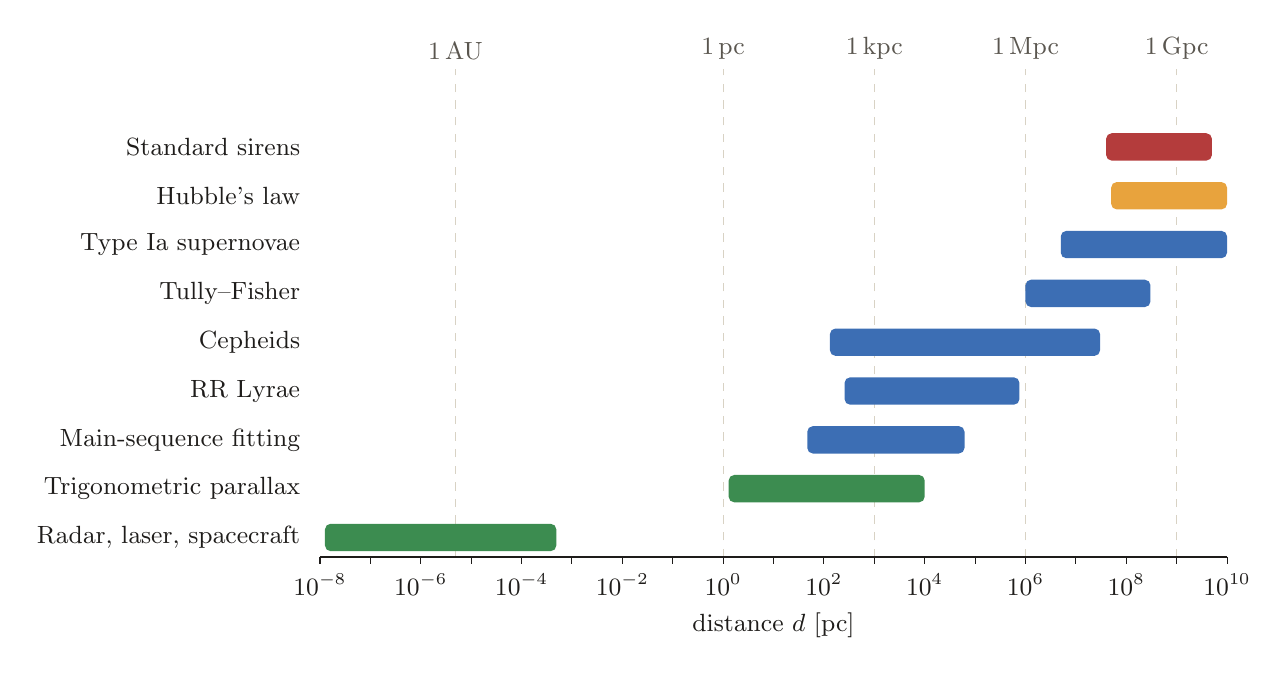
\begin{tikzpicture}[x=0.64cm,y=0.62cm,font=\small]
  \def\xmin{-8}\def\xmax{10}
  % unit lines
  \foreach \u/\lab in {-5.31/1\,AU, 0/1\,pc, 3/1\,kpc, 6/1\,Mpc, 9/1\,Gpc}{
    \draw[linecol,dashed] (\u,-0.4) -- (\u,9.6);
    \node[above,muted] at (\u,9.6) {\lab};
  }
  % axis
  \draw[thick,ink] (\xmin,-0.4) -- (\xmax,-0.4);
  \foreach \k in {-8,...,10}{\draw[ink] (\k,-0.4) -- (\k,-0.55);}
  \foreach \k in {-8,-6,...,10}{\node[below,ink] at (\k,-0.55) {$10^{\k}$};}
  \node[below,ink] at (1,-1.35) {distance $d$ [pc]};
  % bars: y, left, right, colour, label
  \foreach \y/\a/\b/\c/\lab in {
      0/-7.90/-3.31/colthree/{Radar, laser, spacecraft},
      1/0.11/4.00/colthree/{Trigonometric parallax},
      2/1.67/4.79/coltwo/{Main-sequence fitting},
      3/2.41/5.88/coltwo/{RR Lyrae},
      4/2.12/7.48/coltwo/{Cepheids},
      5/6.00/8.48/coltwo/{Tully--Fisher},
      6/6.70/10.00/coltwo/{Type Ia supernovae},
      7/7.70/10.00/sunyellow/{Hubble's law},
      8/7.60/9.70/colone/{Standard sirens}}{
    \fill[\c,rounded corners=2pt] (\a,\y-0.28) rectangle (\b,\y+0.28);
    \node[left,ink,anchor=east] at (\xmin-0.2,\y) {\lab};
  }
\end{tikzpicture}
\end{document}
